\documentclass{article}
\usepackage[utf8]{inputenc}
\usepackage{amsmath}
\usepackage{amssymb}
\usepackage{graphicx}
\usepackage{caption}
\usepackage{subcaption}
\usepackage{epstopdf}
\usepackage{url}
\usepackage{float}
\usepackage{array}
\usepackage[export]{adjustbox}

\usepackage{todonotes}
\usepackage{bytefield}

\usepackage{geometry}
\geometry{
    a4paper,
    total={170mm,257mm},
    left=30mm,
    right=30mm,
    top=15mm,
}

% code listings
\usepackage{listings}
\lstset{
    language=C++,
    numbers=left,
    basicstyle=\footnotesize\ttfamily,
    breaklines=true,
    tabsize=4,
    keepspaces=true,
    columns=flexible,
    frame=single,
    morekeywords={matlab2tikz},
    keywordstyle=\color{blue},
    morekeywords=[2]{1}, keywordstyle=[2]{\color{black}},
    identifierstyle=\color{black},
    stringstyle=\color{mylilas},
    commentstyle=\color{mygreen},
    showstringspaces=false,%without this there will be a symbol in the places where there is a space
    numberstyle={\tiny \color{black}},% size of the numbers
    numbersep=9pt, % this defines how far the numbers are from the text
    emph=[1]{for,end,break},emphstyle=[1]\color{red},
    %emph=[2]{word1,word2}, emphstyle=[2]{style},    
}
\usepackage{color} %red, green, blue, yellow, cyan, magenta, black, white
\definecolor{mygreen}{RGB}{28,172,0} % color values Red, Green, Blue
\definecolor{mylilas}{RGB}{170,55,241}

\usepackage{enumitem}
\newlist{registerdescription}{description}{2}
\setlist[registerdescription]{labelwidth=1.5cm,leftmargin=!,font=\normalfont}

\title{Embedded Systems Mini-Project\\
 Avalon Camera Controller Implementation on Cyclone V FPGA}
\author{
  Snoeijs, Jan\\
  EPFL\\
  \texttt{jan.snoeijs@epfl.ch}
  \and
  Spieler, Michael\\
  EPFL\\
  \texttt{spieler.micheal@epfl.ch}
  }

\date{January 2018}

\begin{document}

\maketitle

\section{Introduction}
In this document we present our implementation of the design proposed in our report of laboratory 3, on the Cyclone V FPGA using a NIOS II processor and an Avalon Bus. We will more specifically detail the changes we made compared to the theoretical design and explain the structure of the hardware and the software source files, as well as the top-level Qsys connectivity.

\section{Hardware structure}

In this section we present the hardware structure of our implemented design and compare the small differences with the theoretical design.

\subsection{Custom Component: Avalon Camera Controller}

The implemented hardware architecture of the custom camera controller is shown in Figure \ref{fig:CameraComponent}. We made some changes compared to the theoretical version of the design; specifically, we added (green) and removed (red) some top-level connections, put the LineFIFO out of the Camera Interface component and the PLL outside our Custom Component (connected as an additional component in Qsys). These changes are induced by the hierarchy we chose for our VHDL files, and for simplicity the routing of all internal components was done in our custom component top-level file. Concerning the PLL, we removed it from our component because its clock output was always zero if we integrated it.

\begin{figure}[H]
\centering
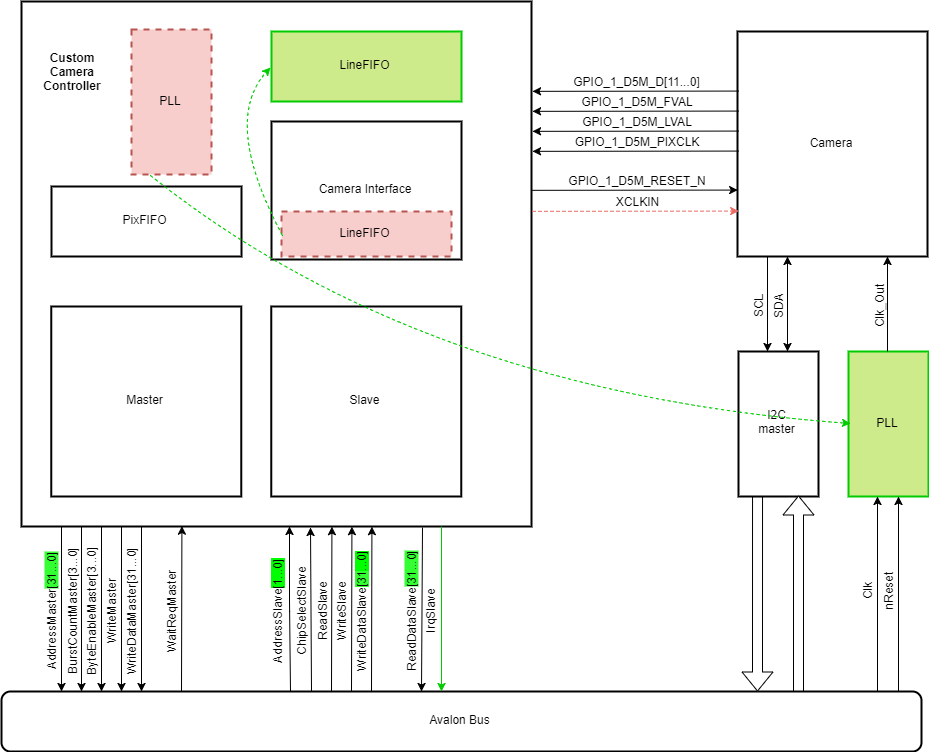
\includegraphics[scale=0.4]{images/CameraComponent.png}
\caption{Custom avalon camera controller --- Implemented architecture and modifications}
\label{fig:CameraComponent}
\end{figure}

\subsection{Integration of Custom Component in FPGA}

Figure \ref{fig:FpgaSystem} shows the full system architecture implemented on the Cyclone V FPGA.

\begin{figure}[H]
\centering
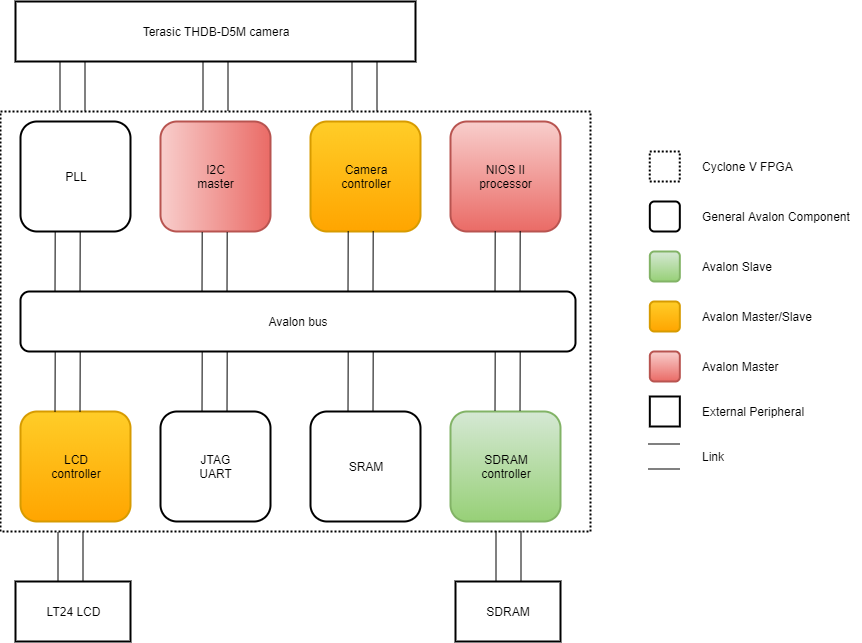
\includegraphics[scale=0.45]{images/FpgaSystem.png}
\caption{FPGA Full System Architecture --- Implementation on Cyclone V}
\label{fig:FpgaSystem}
\end{figure}

\section{Hardware Implementation}

We present the detailed implementation of the hardware architecture shown in the previous section. 

\subsection{Avalon Slave Component}
The updated Avalon slave component block diagram is shown in figure \ref{fig:avalon_slave}. 
We made some changes since the original design:
\begin{itemize}
    \item The Start Image Interrupt was removed because it was not useful on the software side.
    \item The \verb'MasterEnable' signal was removed, since it was not required.
    \item The \verb'AddressUpdate' signal was moved to the Camera Interface component because we changed the behaviour such that the DMA component updates it's destination address on every new incoming frame.
    \item The image address in the \verb'IAR' register can be updated anytime. For an ongoing transfer the frame will be stored at it's initial address and an update will be applied for the next frame.
    \item We defined that only 32bit word access are allowed to the registers to simplify our design.
\end{itemize}

\begin{figure}[H]
\centering
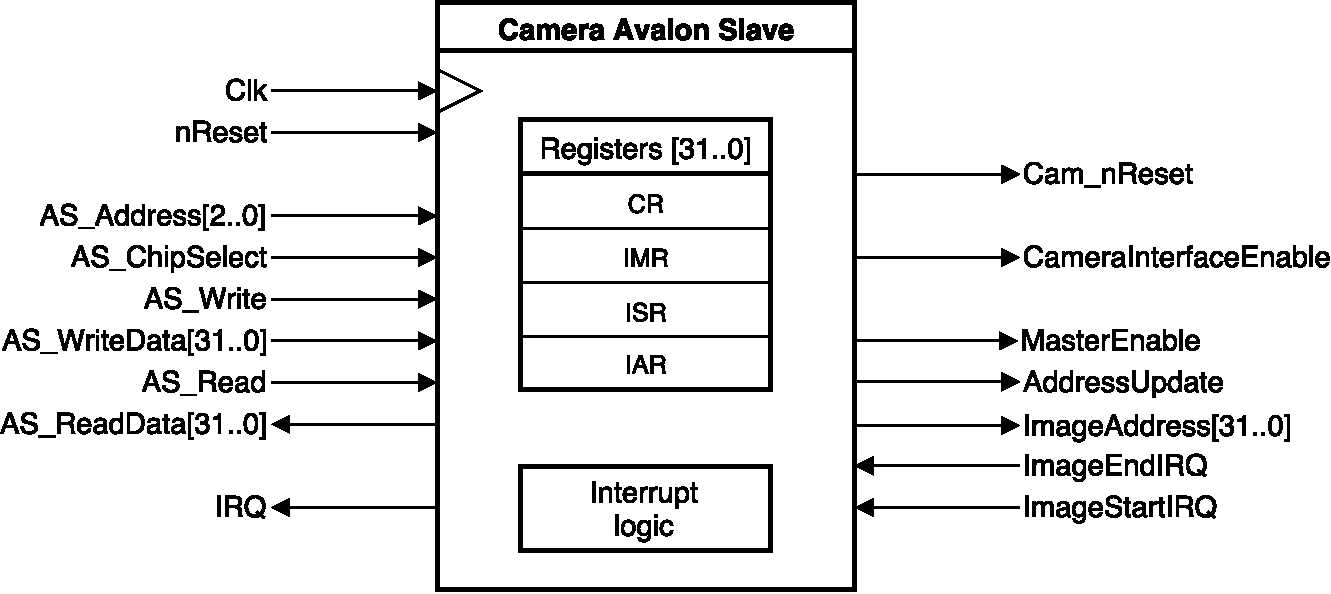
\includegraphics[width=\textwidth]{images/CameraAvalonSlave.pdf}
\caption{Camera Avalon slave block diagram}
\label{fig:avalon_slave}
\end{figure}

\subsubsection{VHDL structure}

The avalon slave has following VHDL processes:
\begin{description}[align=right, leftmargin=*,labelindent=2cm]
\item[pRegWr] Handles Avalon write access to internal registers.
\item[pRegRd] Handles Avalon read access to internal registers.
\item[pInt] Generates an interrupt on \verb'IRQ' signal when the \verb'ImageEndIrq' line is asserted and the interrupt is enabled in \verb'IMR' Interrupt Mask Register.
\end{description}

\subsubsection{Interrupts}
The camera controller provides an interrupt for when a frame is received. It can be enabled using the Interrupt Mask Register (IMR). The correct functioning of the interrupt was successfully tested in the software running on NIOS-II\footnote{There was a minor issue that the Altera NIOS-II BSP generator provided false interrupt numbers in the system.h file (which were all set to -1). Thus, we took the interrupt number from Qsys, which then worked fine.}.

\subsection{Camera Controller Component}
The updated Avalon slave component block diagram is shown in figure \ref{fig:avalon_slave}. 
We made some changes since the original design:
\begin{itemize}
    \item The \verb'AddressUpdate' signal was moved to the Camera Interface component because we changed the behaviour such that the DMA component updates it's destination address on every new incoming frame.
    \item The signals \verb'LineFIFOclear' and \verb'PixFIFOclear' were added to ensure a defined FIFO state on every new frame reception.
    \item We removed the down-sampling since it was not necessary (see explanation below).
\end{itemize}

\begin{figure}[H]
\centering
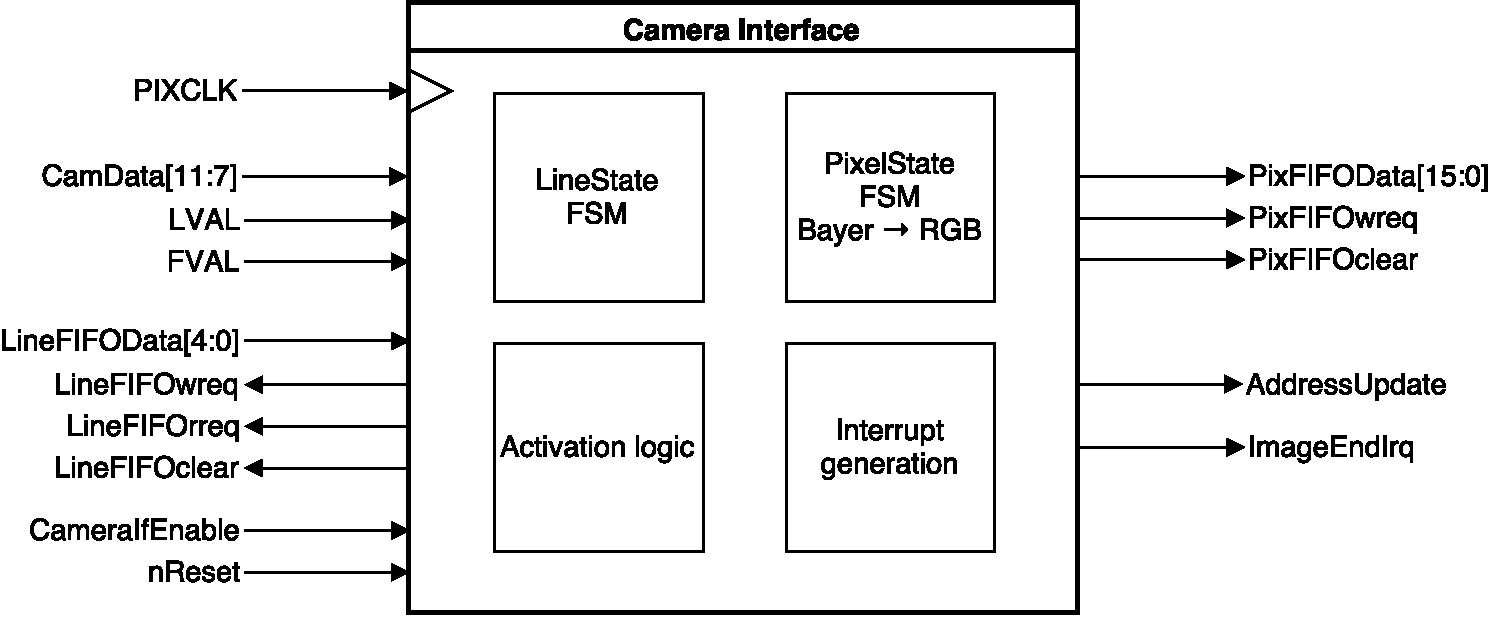
\includegraphics[width=\textwidth]{images/CameraInterface.pdf}
\caption{Camera interface block diagram}
\label{fig:camera_interface}
\end{figure}

\subsubsection{Data reception}

The camera data transmission is summarized in figure \ref{fig:camera_signals}. Figure \ref{fig:image_transmission} shows the signals of one frame transmission and figure \ref{fig:line_transmission} gives a more detailed view of the line transmission.

\begin{figure}[H]
\begin{subfigure}[b]{\textwidth}
\centering
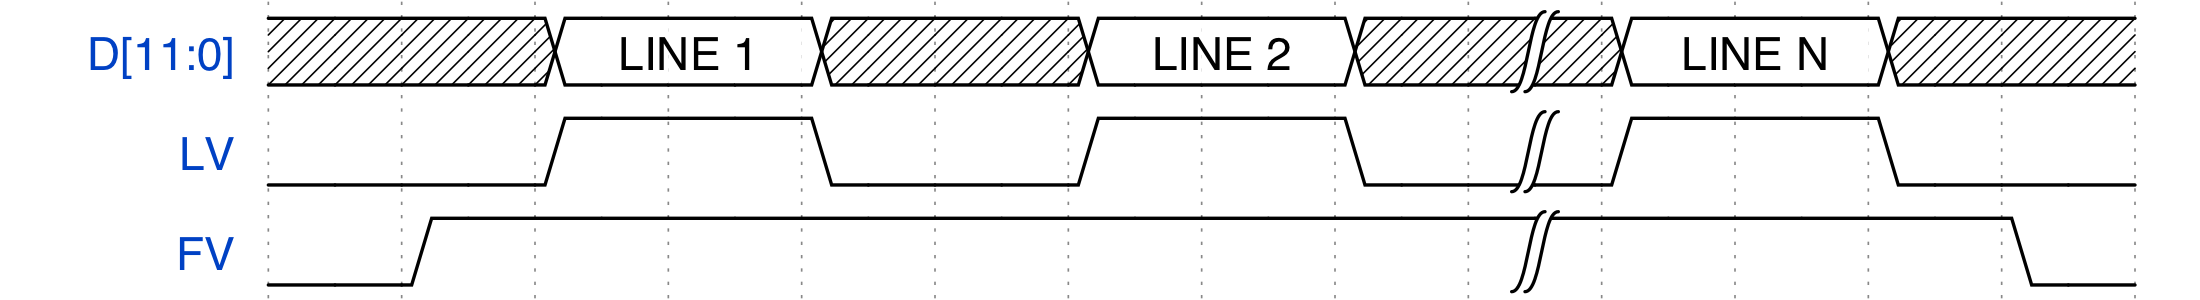
\includegraphics[width=\textwidth]{images/image_transmission.png}
\caption{Camera frame transmission with LineValid and FrameValid signals.}
\label{fig:image_transmission}
\end{subfigure}

\begin{subfigure}[b]{\textwidth}
\centering
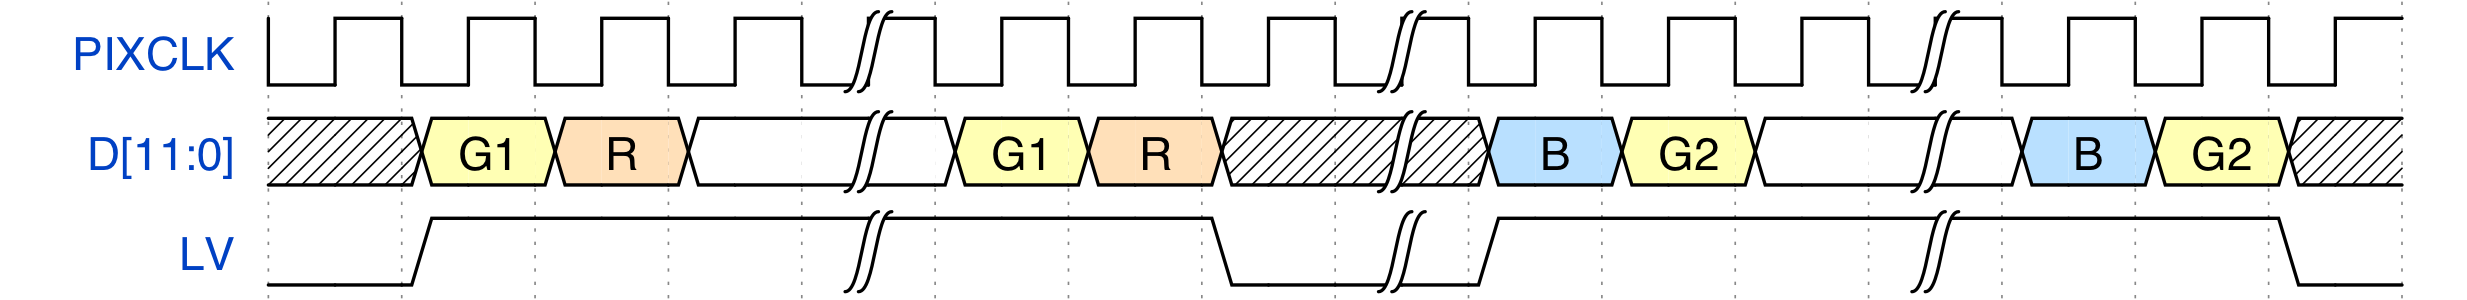
\includegraphics[width=\textwidth]{images/line_transmission.png}
\caption{Transmission of one pixel line transmission composed of two sensor lines.}
\label{fig:line_transmission}
\end{subfigure}
\caption{Camera signals wave diagram.}
\label{fig:camera_signals}
\end{figure}

Figure \ref{fig:camera_interface_signals} shows the timing diagram of the input and output signals of the final camera interface. 

\paragraph{Note:}
One of the changes from the original design was that we removed the down-sampling of the image.
This was due to the fact that with our chosen camera configuration the received frame consists of 640x480 sensors instead of pixels.
As a result, the image after the conversion from Bayer to RGB has 320x240 pixels, which is already the right dimension.
Thus, there is no need for the down-sampling the frame, which we then removed from the final implementation. This means that every received pixel is directly forwarded to the DMA controller.

\begin{figure}[H]
\centering
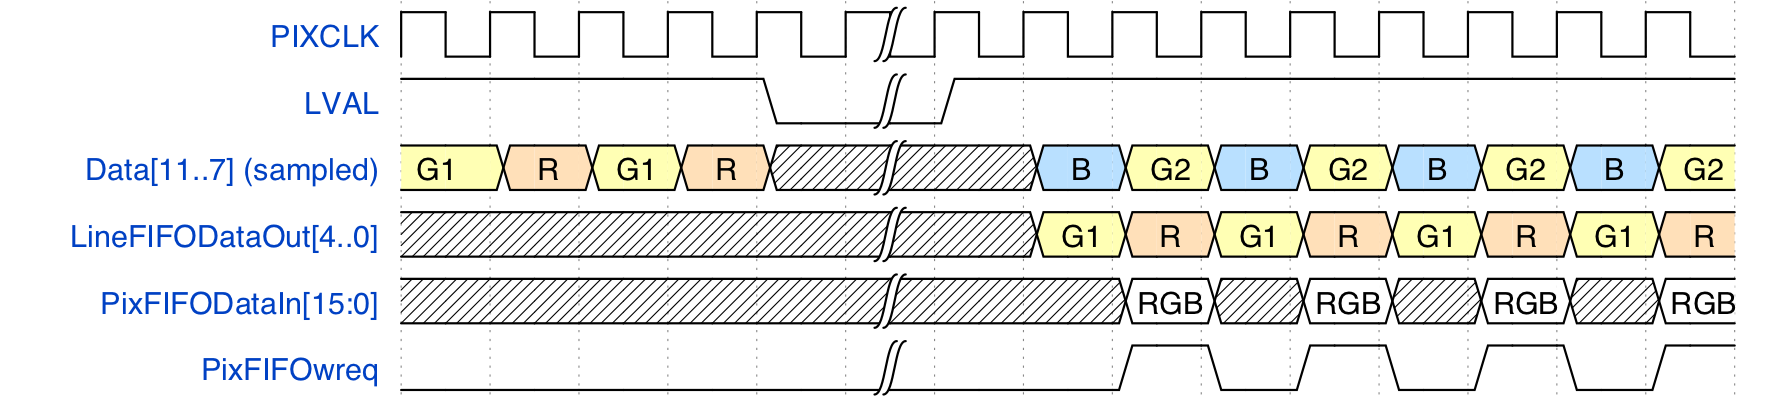
\includegraphics[width=\textwidth]{images/camera_interface_data_signals.png}
\caption{Camera interface signals transforming the Bayer pattern to a RGB pixel.}
\label{fig:camera_interface_signals}
\end{figure}

\subsubsection{Finite State Machine}
Figure \ref{fig:camera_interface_fsm} shows the 3 internal Finite State Machines in the Camera Interface.
The first one is for activation the interface through the \verb'CameraInterfaceEnable' signal. It set's the component into the \verb'ACTIVE' state when the first start of frame is received while \verb'CameraInterfaceEnable' is asserted. This guarantees that only entire images are received even if the interface is enabled during a frame transmission.
The second FSM handles the sensor line states corresponding to the camera LVAL signal.
It alternates between the states \verb'LBUFFER' for buffering a line into LineFIFO and \verb'LPROCESS' for processing the incoming line with the buffered line.
The third FSM handles the pixel processing during the \verb'LPROCESS' state.
It alternates between \verb'PBUFFER' where the pixel data are cached and \verb'PWRITE' where the RGB pixel is generated and written into the PixelFIFO.

\begin{figure}[H]
\centering
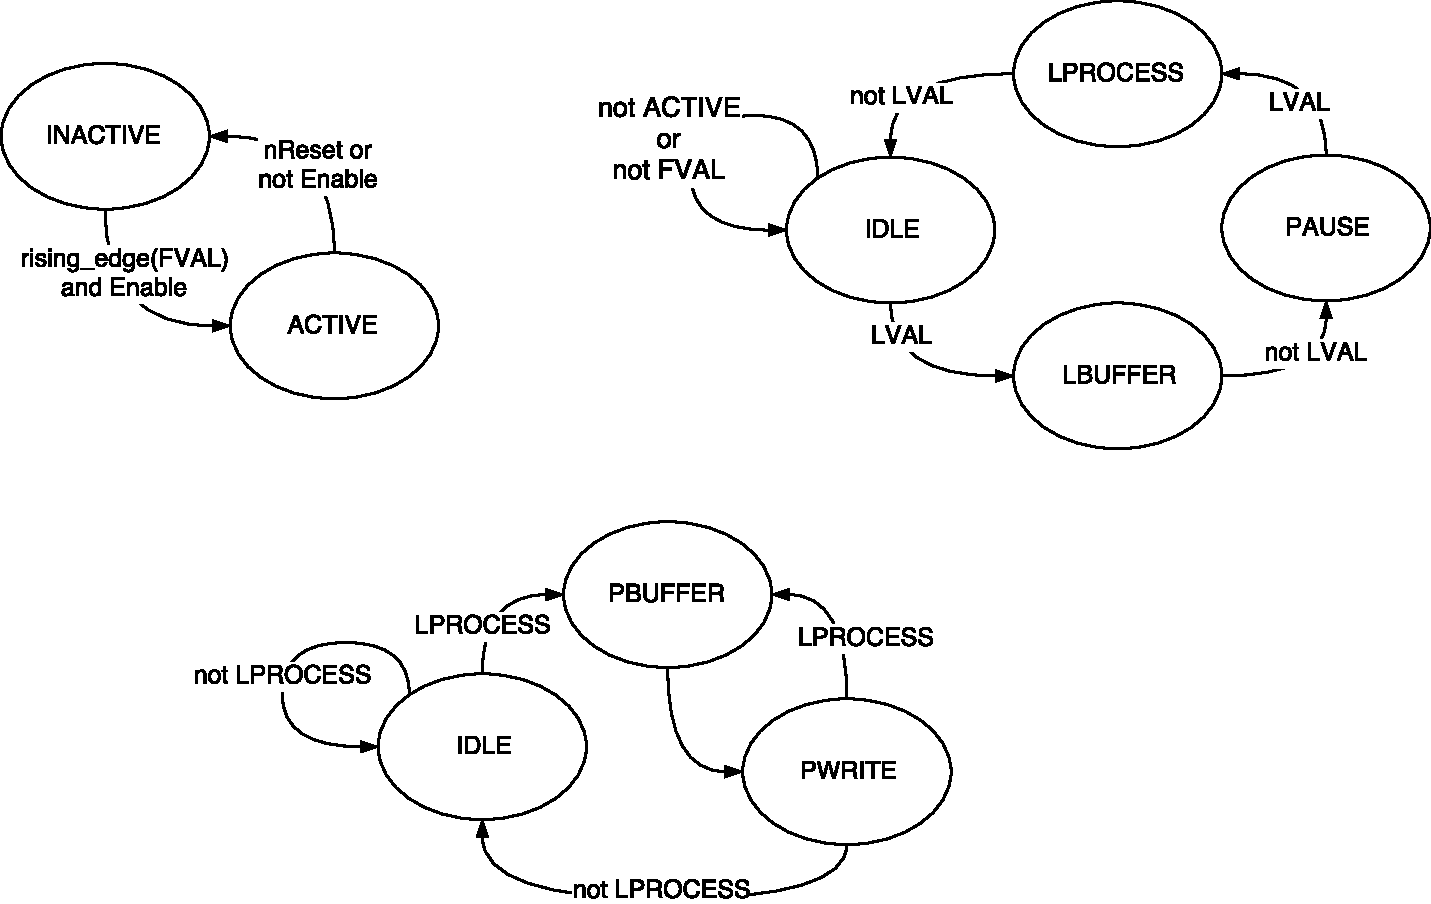
\includegraphics[width=\textwidth]{images/CameraInterfaceFSM.pdf}
\caption{Camera interface Finite State Machine transition schema.}
\label{fig:camera_interface_fsm}
\end{figure}

Figur \ref{fig:camera_rgb} illustrates conceptually the process of RGB image combination from the Bayer pattern which depends on the PixelState.
Those steps are realized inside the FSM VHDL process.

\begin{figure}[H]
\centering
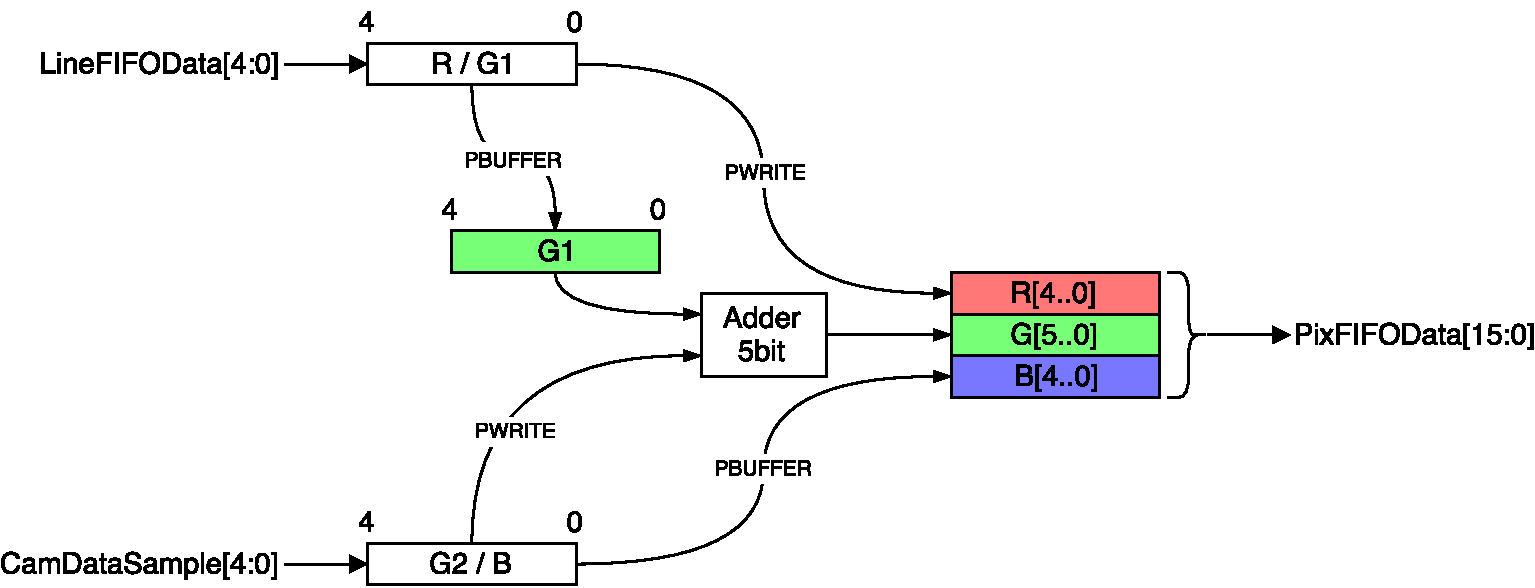
\includegraphics[width=\textwidth]{images/CameraInterfaceBayerToRGB.pdf}
\caption{Bayer pattern to RGB conversion depending on PixelState.}
\label{fig:camera_rgb}
\end{figure}

\subsubsection{VHDL structure}
The camera interface has following VHDL processes:
\begin{description}[align=right, leftmargin=*,labelindent=3cm]
\item[pStateTransition] Makes the state transition of the FSMs synchronous to \verb'PIXCLK'.
\item[pNextStateLogic] Asynchronous process that determines the next states for the FSMs.
\item[pActive] Allows the activation of the camera interface through the CameraInterfaceEnable signal. This process prevents activation during an ongoing frame transmission to ensure receiving valid image data. Furthermore, at the beginning of a new incoming frame, it asserts the signals \verb'PixFIFOaclr', \verb'LineFIFOclear' and \verb'AddressUpdate' to reset the FIFOs and notify the master to copy the image address register from the slave.
\item[pEndIrq] Generates the ImageEnd interrupt.
\end{description}

All signals in the Camera Interface are in the 10MHz PIXCLK domain except for the process pEndIrq which synchronous to the 50MHz main clock domain.

\subsubsection{Timing}

Figure \ref{fig:sim_line} shows the camera interface simulated in the test bench. The signals \verb'Clk', \verb'FValid', \verb'LValid', \verb'CamData' and \verb'LineFIFOData' are provided by the simulation. The signal \verb'PixFIFOData[15:0]' and \verb'PixFIFOwreq' are the output signals. The signals \verb'PixelState' and \verb'LineState' represent the internal states of the finite state machine.

In the shown simulation, we applied the input signal for only one line of 4 pixels. The working principle is the same for any image size. 
We observe a correct state transition of \verb'LineState' through \verb'IDLE', \verb'LBUFFER', \verb'PAUSE', \verb'LPROCESS' and \verb'IDLE' again.
Figure \ref{fig:sim_lprocess} shows that only during \verb'LPROCESS' the \verb'PixelState' FSM is active and alternates between the states \verb'PBUFFER' and \verb'PWRITE'. Those states control the pixel FIFO write request signal \verb'PixFIFOwreq' to write \verb'PixFIFOData' into the FIFO.

\begin{figure}[H]
\centering
\begin{subfigure}[b]{\textwidth}
\centering
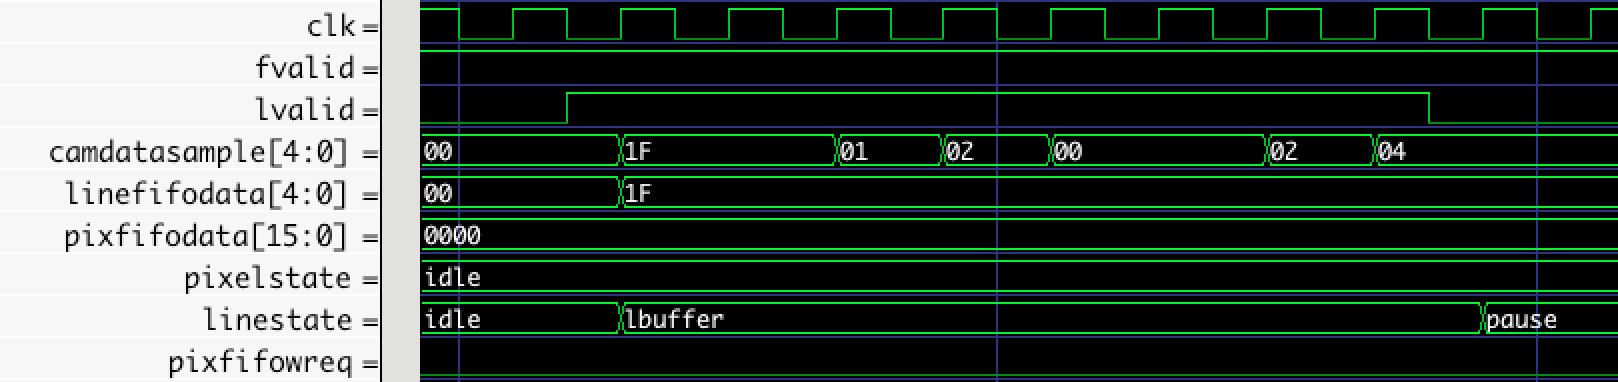
\includegraphics[width=\textwidth]{images/cam_interface_sim_lbuffer.png}
\caption{Simulation of the line buffer phase, where the first sensor line is stored in the LineFIFO.}
\label{fig:sim_lbuffer}
\end{subfigure}
~
\begin{subfigure}[b]{\textwidth}
\centering
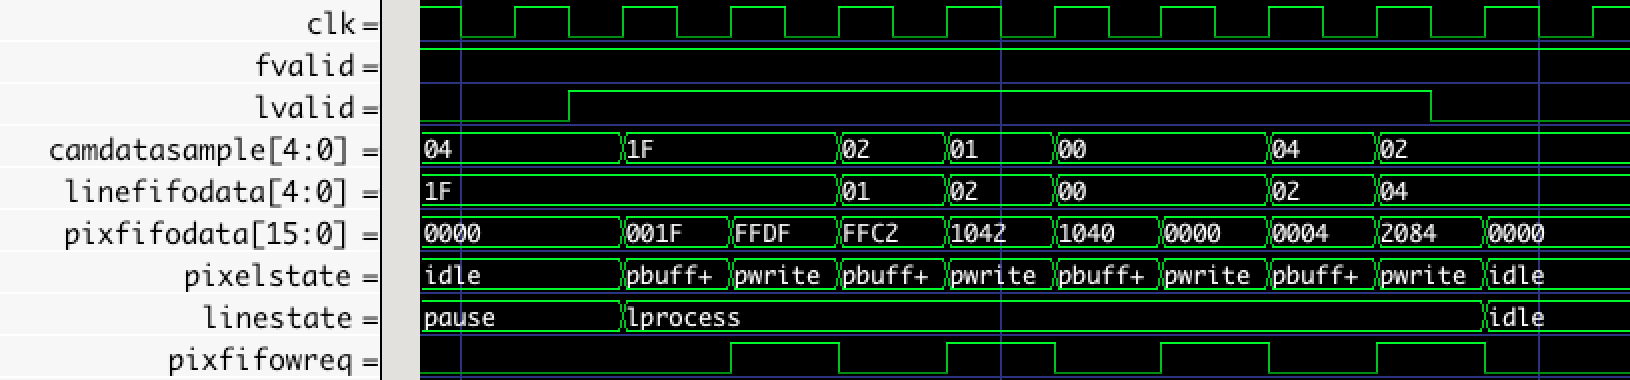
\includegraphics[width=\textwidth]{images/cam_interface_sim_lprocess.png}
\caption{Simulation of the line process phase, where the bayer pattern is converted into RGB format.}
\label{fig:sim_lprocess}
\end{subfigure}
\caption{Simulation of the camera interface line reception.}
\label{fig:sim_line}
\end{figure}

We verified the camera interface behaviour by exposing the internal states on GPIOs and capturing them with a logic analyzer. 

Figure \ref{fig:capture_line_state} shows the state transition of \verb'LineState(1..2)' at the beginning of an frame transfer. It controls the signals \verb'LineFIFOwreq' and \verb'LineFIFOrreq' for writing to or respectively reading from the line FIFO.

Figure \ref{fig:capture_pixel_state} shows the state transition of \verb'PixelState(1..2)' during \verb'LPROCESS'. It controls the signals \verb'PixFIFOwreq' and \verb'PixFIFOData' to write the processed RGB data into the pixel FIFO.

\begin{figure}[H]
\centering
\begin{subfigure}[b]{\textwidth}
\centering
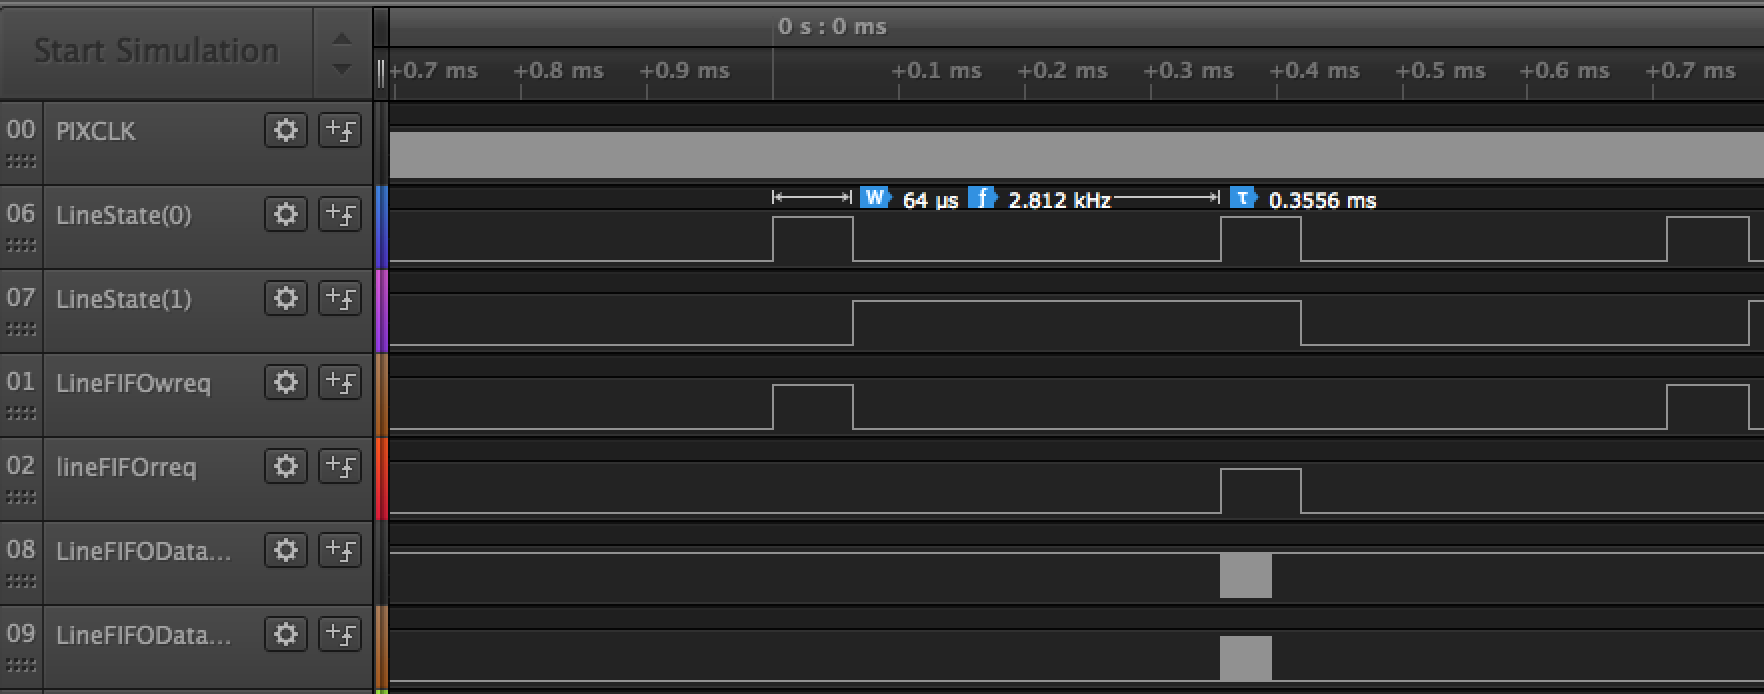
\includegraphics[width=0.9\textwidth]{images/camera_interface_capture_line_state.png}
\caption{LineState capture.}
\label{fig:capture_line_state}
\end{subfigure}
~
\begin{subfigure}[b]{\textwidth}
\centering
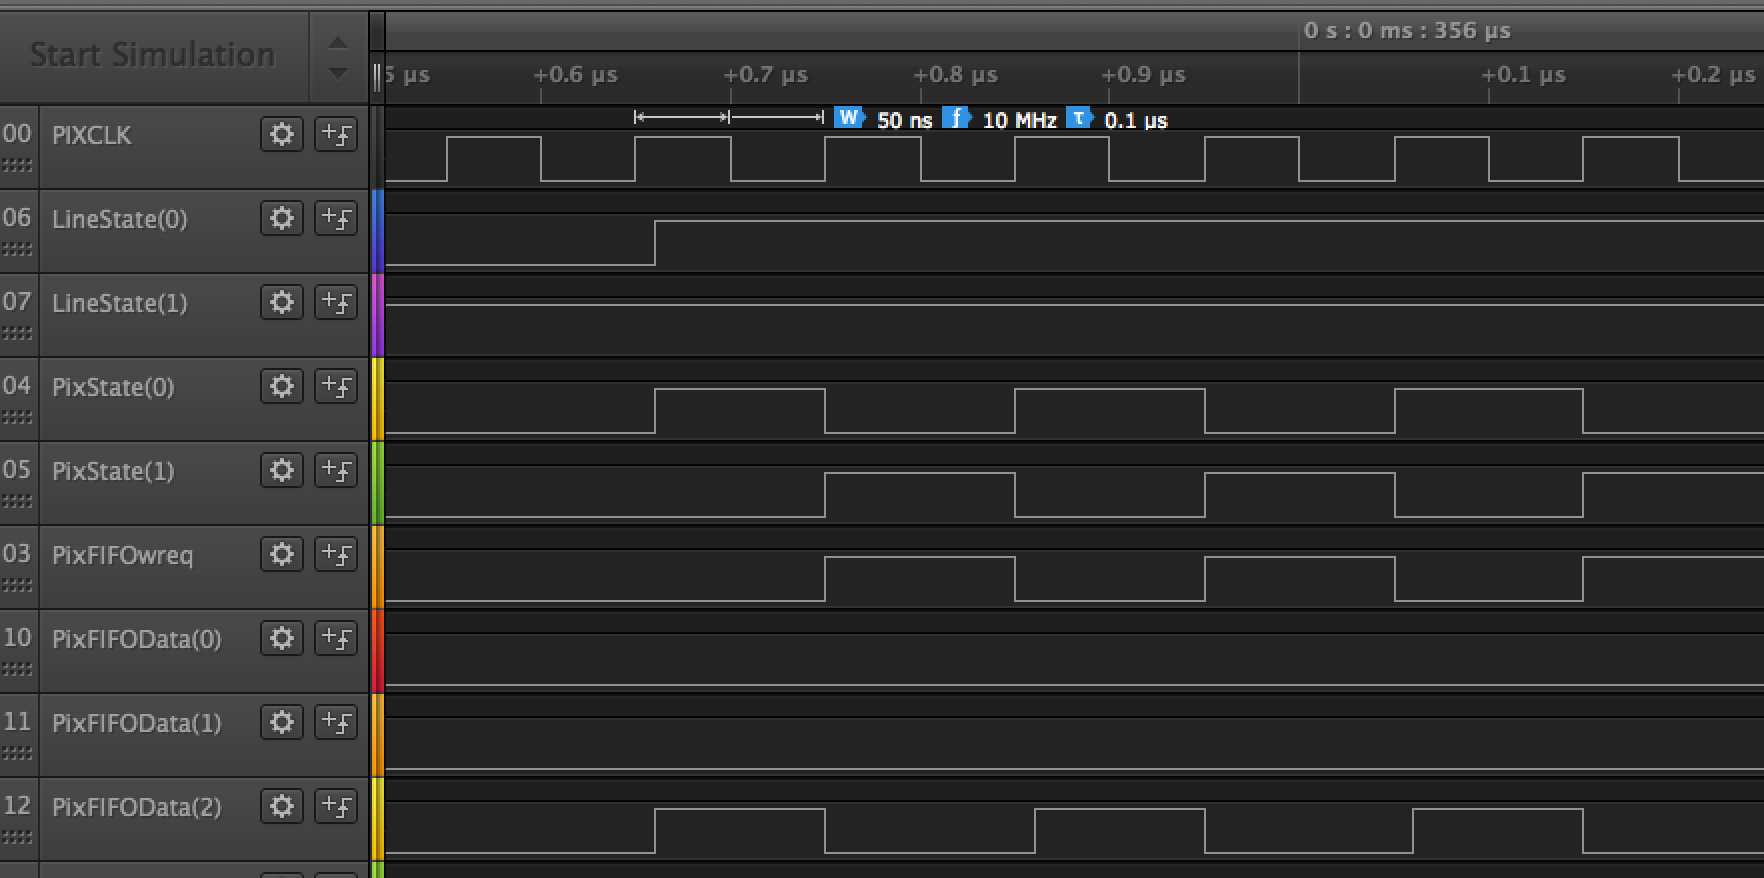
\includegraphics[width=0.9\textwidth]{images/camera_interface_capture_pixel_state.png}
\caption{PixelState capture.}
\label{fig:capture_pixel_state}
\end{subfigure}
\caption{Capture of the line reception.}
\label{fig:capture_interface_states}
\end{figure}

\subsection{Avalon Master component}

The master component reads the data from the dual-clocked PixFIFO and writes in the SDRAM through burst transfers on the Avalon bus. The slave component transmits the memory address of the start of the image. During one burst, 8 32-bit words are sent sequentially to the memory. The component's behavior is controlled by a tri-state FSM which generates the necessary Avalon signals which are necessary for a burst transfer. For example, the outputting of the Avalon address and the dependency to input signal \verb'waitreq' are handled by this state machine. 

\begin{figure}[H]
\centering
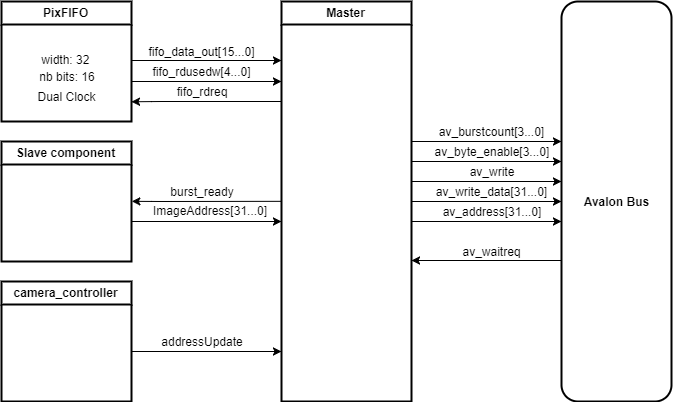
\includegraphics[scale=0.6]{images/MasterGeneral.png}
\caption{Master component --- Interconnects}
\label{fig:MasterGeneral}
\end{figure}

\subsubsection{Finite state machine description}

The FSM is in \verb'IDLE' state until the PixFIFO (32 x 16-bits) gets filled with atleast 16 pixels (16 lines of 16 bits). Between the theoretical design and the implementation we chose to increase the width of the PixFIFO. In the implementation, the state machine is triggered by the \verb'rdusedw[4...0]' signal instead of by the \verb'fifo_full' signal, which should be more robust to data losses in cases of a long wait time on the avalon side. An extra state was added to the finite state machine so that the data transfers in a bursts are consecutive and not interrupted by a processing cycle as that would have been the case with only 2 states. In fact, in the theoretical design we overlooked the fact that only one 16-bit data is available at the same time at the output of the FIFO. Thus the added state (\verb'STORE') actually stores the data contained in the FIFO into a register where all the data is available in parallel. We unfortunately first wrote the master VHDL before realizing that the data can have a different format at the input and output of an Altera FIFO, which would have saved us some logic in the master component. Nevertheless, our implementation of this logic should be functionally correct. Finally the \verb'WRITE' is the state in which the burst transfers are executed and is similar to the one presented in the theoretical design.

\begin{figure}[H]
\centering
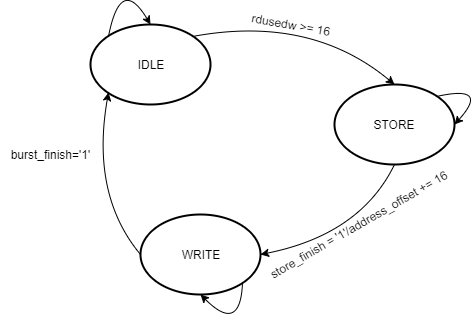
\includegraphics[scale=0.45]{images/MasterFSM.png}
\caption{Master component --- Modified finite state machine}
\label{fig:MasterFSM}
\end{figure}

\begin{figure}[H]
\centering
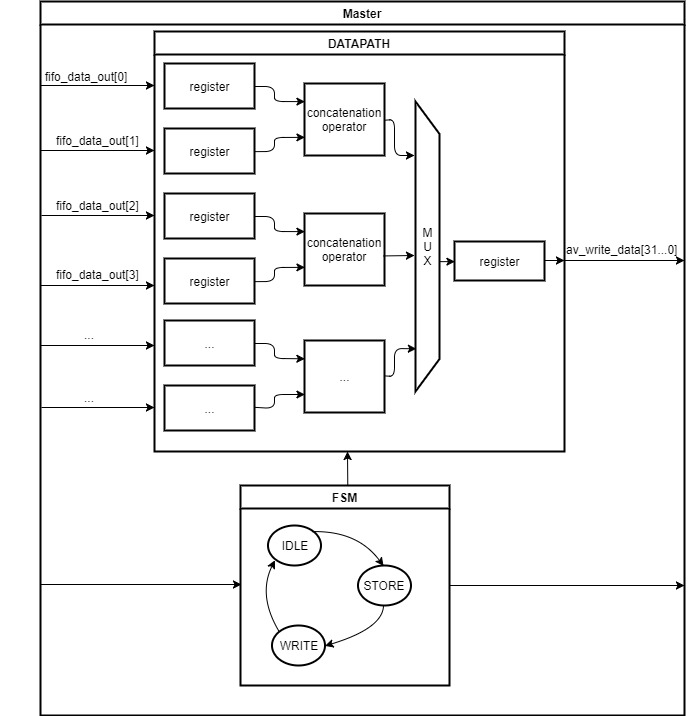
\includegraphics[scale=0.6]{images/MasterInside.png}
\caption{Master --- Internal structure of the datapath}
\label{fig:MasterInside}
\end{figure}

\subsubsection{Timing}

The same timings as presented in theory were observed in the results of Modelsim simulations and also with the logic analyzer. In the theoretical design we misinterpreted the \verb'byte_enable' signal. Since we send 32-bit words in parallel, all the bytes are assumed valid and thus \verb'byte_enable' should always  be \verb'1111' (If doing writes of only 32bit words, the signal could even be omitted to our knowledge). Figures \ref{fig:MasterAvalonTiming} and \ref{fig:MasterFifoTiming} show the simulation results of the master component working isolated from the rest of the design by providing arbitrary FIFO output signals as a stimuli.
\begin{figure}[H]
\centering
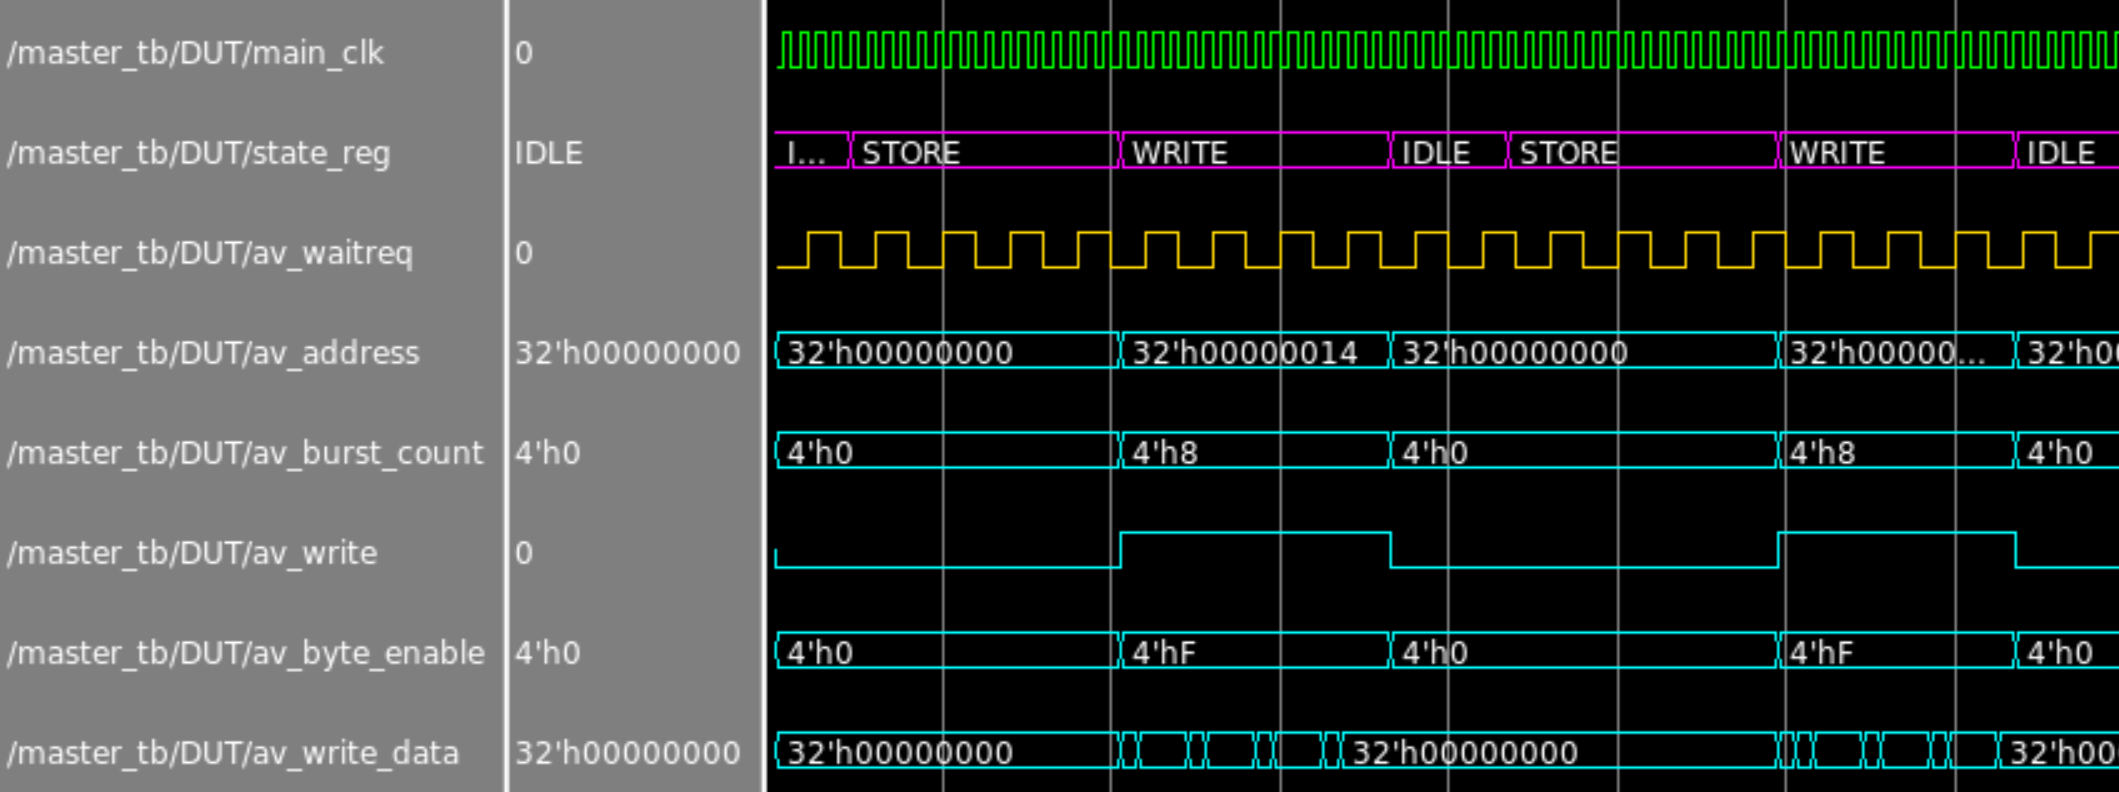
\includegraphics[scale=0.65]{images/MasterAvalonTiming.png}
\caption{Results of Modelsim simulation of master component --- Avalon signals}
\label{fig:MasterAvalonTiming}
\end{figure}

\begin{figure}[H]
\centering
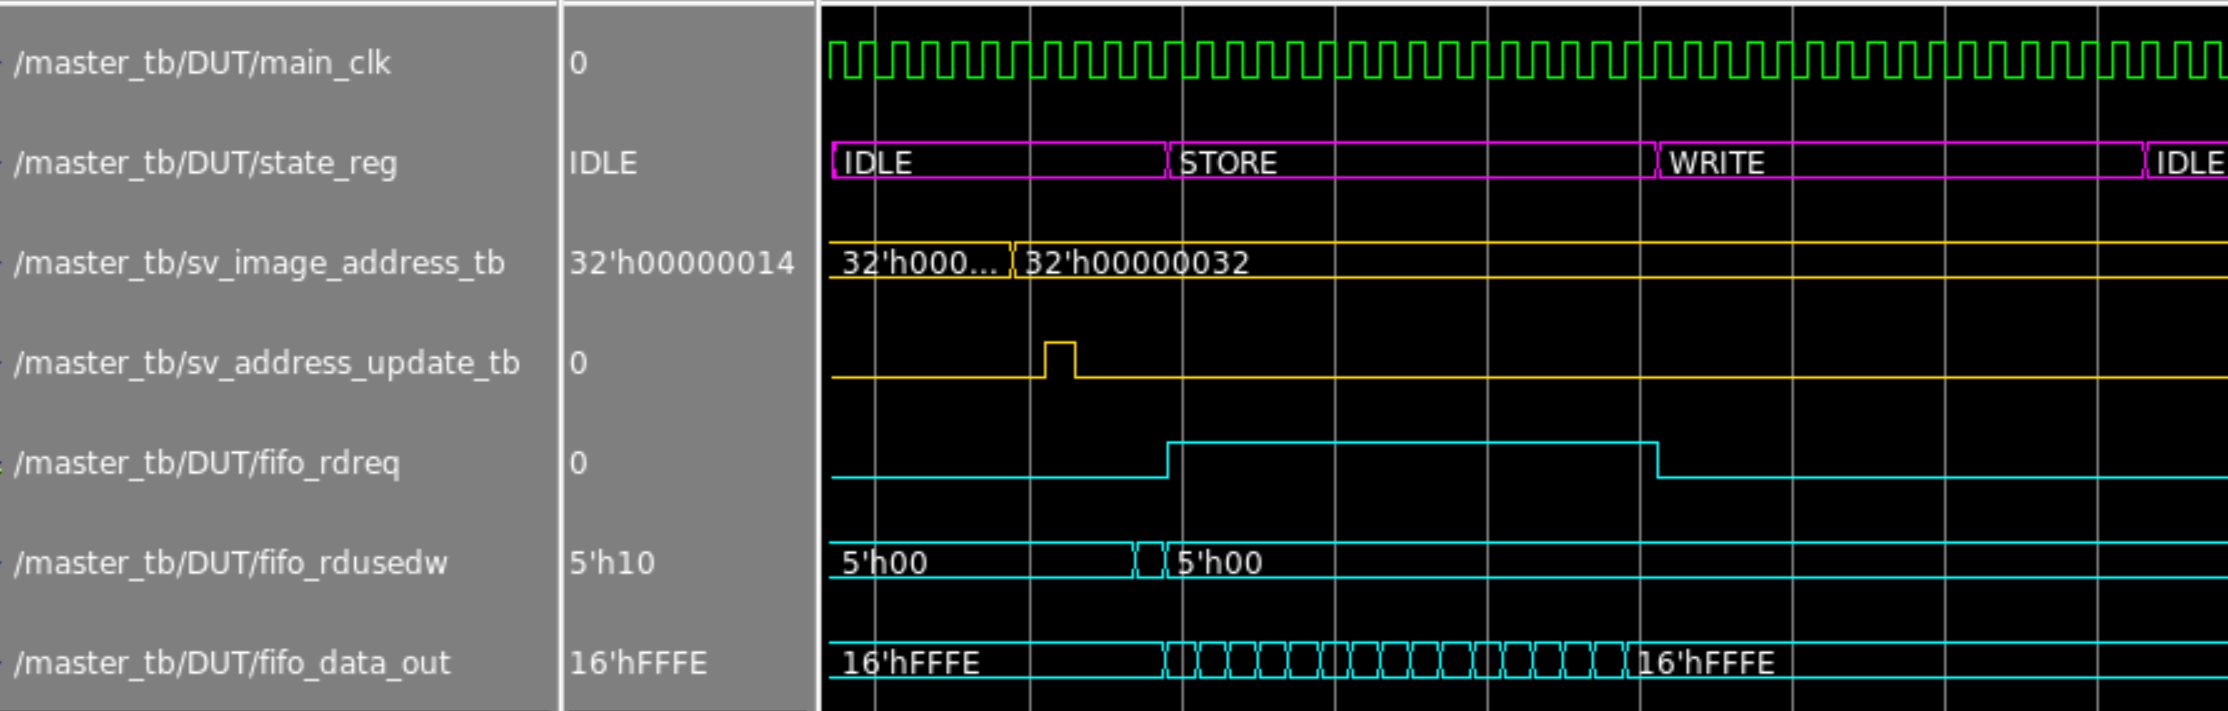
\includegraphics[scale=0.62]{images/MasterFifoTiming.png}
\caption{Results of Modelsim simulations of master component --- PixFIFO signals}
\label{fig:MasterFifoTiming}
\end{figure}

During debugging we verified the timing of the component in the real system by exposing the Avalon master signals on free GPIOs and capturing them with a logic analyzer.
Figure \ref{fig:burst_capture} shows the capture of the most important signals. We observe that the waitrequest is asserted for the first clock cycle and it is correctly considered by the Avalon master, delaying the burst for one more clock cycle. The burst finished after 8 clock cycles by de-asserting the Write signal.

\begin{figure}[H]
\centering
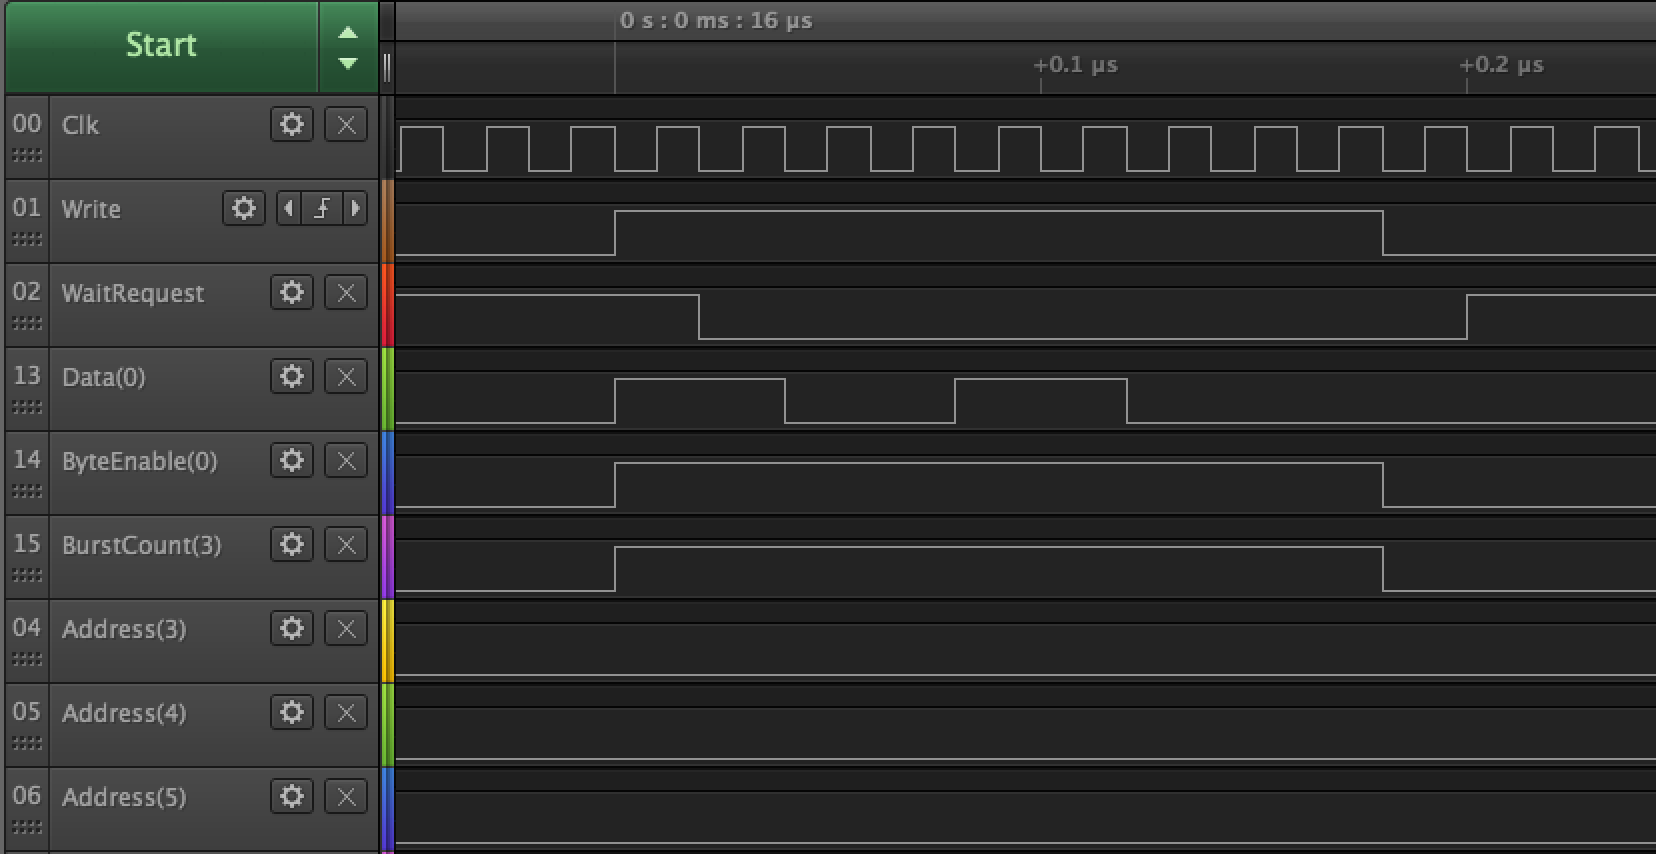
\includegraphics[width=0.9\textwidth]{images/avalon_burst_capture1.png}
\caption{Logic analyzer capture of one Avalon burst write running in the complete system.}
\label{fig:burst_capture}
\end{figure}

\subsubsection{Limitations}
One known limitation of the interface is that if the camera is wrongly configured for a different frame size, a buffer overrun can occur.
This is due to the fact that we do not count the number of received pixels and therefore there is no boundary check.
Thus, the DMA always writes the whole data stream into memory even if it does not fit the image buffer. \footnote{This is a possible point of improvement: We could add a counter with an image size register to the component. This would allow us to check the number of bytes received and to stop when the maximum is reached.}

\subsection{Altera FIFO components configuration}

Our design comprises two FIFOs provided by ALTERA. The table \ref{tab:fifoconf} shows how we configured LineFIFO, used by our camera interface component and PixFIFO, the input of the master component. The \verb'rdreq' signal acts like an acknowledge in both our FIFOs, this allows to have no delay between the moment when \verb'rdreq' is asserted and the actual readout of the data (show ahead option)
\begin{table}[H]
\centering
\caption{ALTERA FIFOs configuration}
\vspace{0.2 cm}
\begin{tabular}{|c|c|c|}
\hline
    Configurations & LineFIFO & PixFIFO\\
    \hline
    Width & 2048 & 32 \\
    \hline
    element size (bits) & 5 & 16\\
    \hline
    Clock  & Single & Dual \\
    \hline
    control signals & \verb'almost_full' & \verb'rdusedw[4...0]'\\
    \hline
    \verb'rdreq' & show ahead & show ahead\\
    \hline
\end{tabular}
\label{tab:fifoconf}
\end{table}

%\subsection{Custom Component top-level Connection}

\section{Qsys Configuration and Interconnects}

Finally, our custom \verb'cam_controller' component is inserted in Qsys and connected to the rest of the system.
The Qsys system view is presented in figure \ref{fig:qsys}.
The \verb'cam_controller' component has following connections: a clock, a reset source, NIOS-II data master to the Avalon slave, the Avalon master to the \verb'address_span_extender' to access the external SDRAM memory and an interrupt sender to the NIOS-II.
The camera and debug signals are exported as a conduit which makes them accessible in the DE0 Nano SoC top level design where we connect them to the GPIOs.

To make the camera work we also needed to added the components I2C for configuration and a PLL delivering a 10MHz clock source source to the camera.

\begin{figure}[H]
\centering
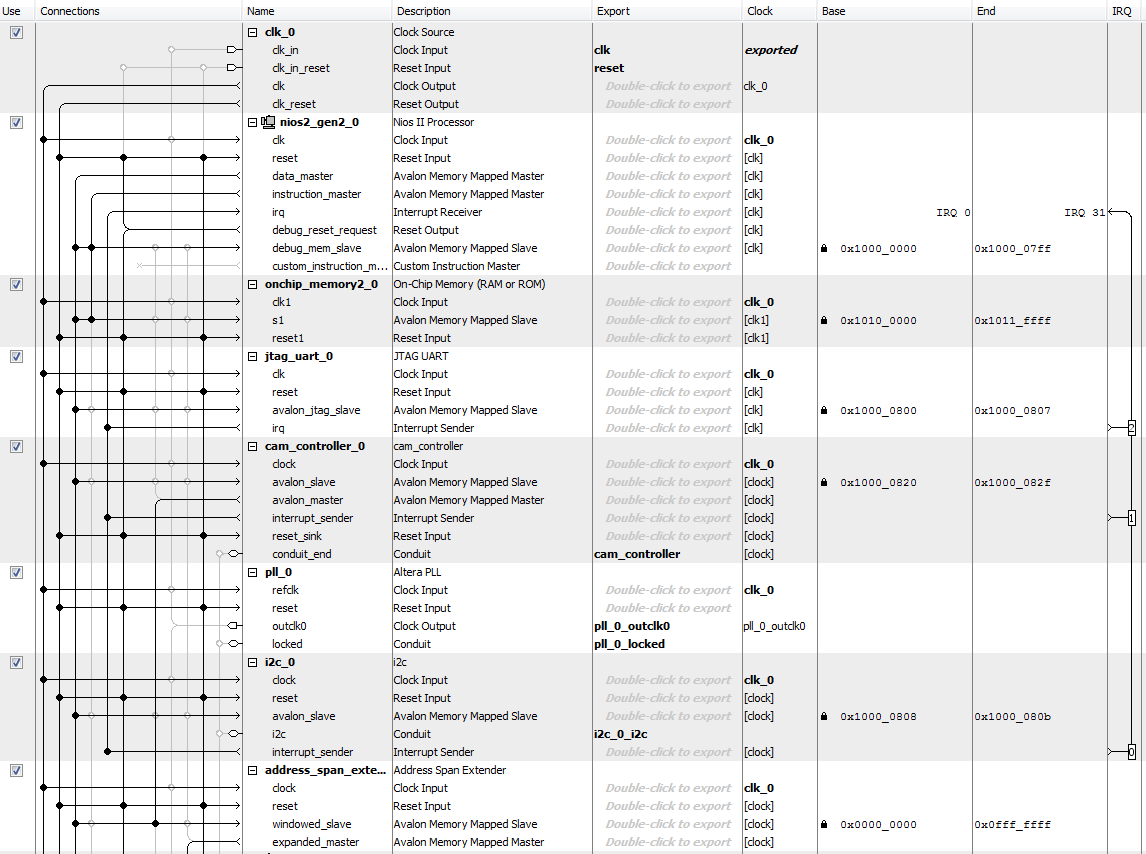
\includegraphics[width=\textwidth]{images/Qsys.png}
\caption{Qsys system view.}
\label{fig:qsys}
\end{figure}

\section{Software on the NIOS-II processor}

\subsection{Camera API description}
The developed camera software allows to receive and store image frames from the camera into a memory buffer. In this part we will go through the camera driver API presented in listing \ref{lst:camera_h} by using an illustrative example setup as shown in listing \ref{lst:example_c}.

\begin{lstlisting}[
    caption=camera.h,
    label=lst:camera_h
]
void camera_enable(void);
void camera_disable(void);
void camera_enable_receive(void);
void camera_disable_receive(void);
void camera_enable_interrupt(void);
void camera_disable_interrupt(void);
void camera_setup(i2c_dev *i2c, uint16_t *buf, void (*isr)(void *), void *isr_arg);
bool camera_image_received(void);
void camera_clear_irq_flag(void);
void camera_set_frame_buffer(uint16_t *buf);
uint16_t *camera_get_frame_buffer(void);
void camera_dump_regs(void);
\end{lstlisting}

First the camera needs to be woken up from reset. The functions \verb'camera_enable()' and \verb'camera_disable()' allow to do this from software.
Then we can configure camera over I2C using the function \verb'camera_setup()'.
It takes as argument the configured I2C driver, a frame buffer pointer where the image needs to be stored and it enables interrupts if an interrupt service routine (ISR) is provided through a function pointer.
In this example we use an interrupt which is explained later. 

Now the camera is running and sending images but we're not receiving anything yet.
We have to enable frame reception through \verb'camera_enable_receive()' to make the camera controller start accepting data.

When an frame is received from the camera, the controller triggers an interrupt and the \verb'camera_interrupt()' routine is called. Ideally the camera interrupt routine is used to hand over a received frame to the LCD controller.
The function \verb'camera_get_frame_buffer()' gives us the pointer to the received frame.
To avoid that the camera controller writes into the frame buffer while it is displayed on the LCD, we can set a new frame buffer using \verb'camera_set_frame_buffer()'.
Finally, we need to clear the interrupt flag to mark the interrupt as served and to prevent the ISR from being called again after return.

For debugging purposes we implemented the function \verb'camera_dump_regs()' to which reads all useful camera configuration registers and prints them to the console.

\begin{lstlisting}[
    caption=example.c,
    label=lst:example_c
]
void example(void)
{
    i2c_dev i2c = i2c_inst((void *) I2C_BASE);
    i2c_init(&i2c, I2C_FREQ);

    camera_enable();

    sleep(1); // give the camera time to boot

    camera_setup(&i2c, IMAGE_BUFFER, camera_interrupt, NULL);
    lcd_setup();

    // start reception
    camera_enable_receive();

    while (1) {
        // do something
    }
}

void camera_interrupt(void *arg)
{
    uint16_t *frame = camera_get_frame_buffer();

    // do something with the frame
    lcd_display_frame(frame);

    // where should the next frame go?
    frame = get_next_frame();
    camera_set_frame_buffer(next_image);

    camera_clear_irq_flag();
}
\end{lstlisting}


Note: Image reception can also be done without using interrupts by polling and clearing the camera controller interrupt flag through the functions \verb'camera_image_received()' and \verb'camera_clear_irq_flag()'.

\subsection{Image downloading on a PC}
To inspect the output image we implemented the function \verb'dump_image()', which makes use of the Altera NIOS host filesystem feature accessible through the debugger. It creates a file on the debugger host file system and dumps the image contents in the simple ASCII PPM image format standard.

\subsection{Interfacing with an LCD}
As illustrated in the example code above, the LCD interface would be relatively straightforward by using the camera interrupt to exchange frame buffers between camera and LCD. Unfortunately, this was not realized because of lack of a working DMA.

\section{Issues encountered}
We encountered a major issue during the implementation of the design which was that we were not able to write data from the master component to the SDRAM memory.
We spent a lot of time trying to figure out what could be the cause of this issue and unfortunately did not manage to find it.
Our debugging process consisted of exporting internal signals of our design to the top-level component and connecting them to GPIO pins of the FPGA, which allowed us to observe their behavior with the logic analyzer.
Specifically, for this issue we checked the following points:

\begin{itemize}
  \item All Avalon burst transfer signals including the address and \verb'wait_request' behave correctly both Modelsim and on logic analyzer after having exported these signals to GPIO pins of the FPGA
  \item The micro-switches of the FPGA are set to the correct position
  \item The SD-Card is configured correctly because we could write to the memory from the software code on NIOS II \item WriteData is non zero
  \item Our custom IP component is connected in Qsys to the address span expander on the windowed slave input, like the NIOS II processor. The address span expander is correctly configured and connected to SDRAM (Same as other groups whoes design is functional)
\end{itemize}

 
\section{Conclusion}
We presented the changes we made to the design during its implementation.
Most of the changes are due to the appearance of unexpected problems when we implemented the design exactly as we presented in Lab 3.
Unfortunately the complete system was not functional on the FPGA because the DMA transfers from the maser component did not work and at some point we ran out of debugging ideas to fix this problem.
Nevertheless, the hardware and software implementation is complete.
Except from the DMA issue, everything seems to be working as designed and the system is ready to be integrated into the full system with Camera and LCD. 

\newpage
\section{Appendix}

\subsection{Camera configuration}
In the function \verb'camera_setup()' we apply following camera configuration:
\begin{itemize}
\item \verb'ROW_SIZE' (R0x03) = 1919, Image row dimension
\item \verb'COLUMN_SIZE' (R0x04) = 2559, Image column dimension
\item \verb'SHUTTER_WIDTH_LOWER' (R0x09) = 3
\item \verb'SHUTTER_WIDTH_UPPER' (R0x08) = 0
\item \verb'ROW_ADDRESS_MODE' (R0x22), Enable row downsampling and binning
    \begin{itemize}
    \item \verb'ROW_BIN' bit[5:4] = 3
    \item \verb'ROW_SKIP' bit[2:0] = 3
    \end{itemize}
\item \verb'COLUMN_ADDRESS_MODE' (R0x23), Enable column downsampling and binning
    \begin{itemize}
    \item \verb'COL_BIN' bit[5:4] = 3
    \item \verb'COL_SKIP' bit[2:0] = 3
    \end{itemize}
\item \verb'VERTICAL_BLANK' (R0x06) = 500, decreases frame rate
\item \verb'PIXEL_CLOCK_CONTROL' (R0x0A), Invert \verb'PIXCLK' polarity
    \begin{itemize}
    \item \verb'INVERT_PIXCLK' bit[15] = 1
    \end{itemize}
\item \verb'OUTPUT_CONTROL' (R0x07), Enable camera
    \begin{itemize}
    \item \verb'CHIP_ENABLE' bit[2] = 1
    \end{itemize}
\end{itemize}

Optional configuration setup which was helpful for debugging:
\begin{itemize}
\item \verb'READ_MODE_2' (R0x20), mirrored image output
    \begin{itemize}
    \item \verb'MIRROR_ROW' bit[15] = 1
    \item \verb'MIRROR_COL' bit[14] = 1
    \end{itemize}

\item \verb'TEST_PATTERN_CONTROL' (R0xA0), Enable test pattern for debugging
    \begin{itemize}
    \item \verb'ENABLE_TEST_PATTERN' bit[0] = 1
    \item \verb'TEST_PATTERN_TYPE' = \verb'TEST_PATTERN_MONOCHROME_VERTICAL_BARS' = 7
    \end{itemize}
\item \verb'TEST_PATTERN_RED' (R0xA2) = 0x080
\item \verb'TEST_PATTERN_GREEN' (R0xA1) = 0xfff
\item \verb'TEST_PATTERN_BLUE' (R0xA3) = 0xA80
\item \verb'TEST_PATTERN_BAR_WIDTH' (R0xA4) = 8
\end{itemize}

\newpage
\subsection{Register map}

\paragraph{Warning:} All registers must be accessed by 32bit word writes.
Any byte or half-word access will result in overwriting the entire register.

\subsubsection{Control Register (CR)}
Address offset: 0x00 \\
Reset Value: 0x00000000 \\
[4mm]
\begin{bytefield}[endianness=big,bitwidth=2.67em]{16}
\bitheader[lsb=16]{16-31} \\
\bitbox{16}{Reserved}
\\
\bitheader{0-15} \\
\bitbox{14}{Reserved} &
\bitbox{1}{CE} &
\bitbox{1}{EN}
\end{bytefield}

\begin{registerdescription}
\item [Reserved] Bits 31:2, read only\\Reserved, read as 0
\item [CE] Bit 1, read/write\\Camera Enable. Controls the camera reset line.\\0: Camera is held in reset.\\1: Camera is enabled.
\item [EN] Bit 0, read/write\\Enable the Camera controller.\\0: Camera controller is disabled all camera signals are ignored.\\1: Camera controller is enabled.\\Note: If the camera controller is enabled while the camera is sending a frame, the ongoing transfer is ignored and the enable takes only effect at the next transfer.
\end{registerdescription}

\subsubsection{Interrupt Mask Register (IMR)}
Address offset: 0x01 \\
Reset Value: 0x00000000 \\
[4mm]
\begin{bytefield}[endianness=big,bitwidth=2.67em]{16}
\bitheader[lsb=16]{16-31} \\
\bitbox{16}{Reserved}
\\
\bitheader{0-15} \\
\bitbox{15}{Reserved} &
\bitbox{1}{EIE}
\end{bytefield}

\begin{registerdescription}
\item [Reserved] Bits 31:1, read only\\Reserved, read as 0
\item [EIE] Bit 0, read/write\\image reception End Interrupt Enable. \\0: Interrupt is inhibited.\\1: Interrupt is generated when the bit EIF=1 in ISR register.
\end{registerdescription}

\subsubsection{Interrupt Status Register (ISR)}
Address offset: 0x02 \\
Reset Value: 0x00000000 \\
[4mm]
\begin{bytefield}[endianness=big,bitwidth=2.67em]{16}
\bitheader[lsb=16]{16-31} \\
\bitbox{16}{Reserved}
\\
\bitheader{0-15} \\
\bitbox{15}{Reserved} &
\bitbox{1}{EIF}
\end{bytefield}

\begin{registerdescription}
\item [Reserved] Bits 31:1, read only\\Reserved, read as 0
\item [EIF] Bit 0, read/write\\End Interrupt Flag. Set by hardware when the image data is completely written to memory. This bit must be cleared by software by writing a 1.
\end{registerdescription}

\subsubsection{Image Address Register (IAR)}
Address offset: 0x03 \\
Reset Value: 0x00000000 \\
[4mm]
\begin{bytefield}[endianness=big,bitwidth=2.67em]{16}
\bitheader[lsb=16]{16-31} \\
\bitbox{16}{IA[31:16]}
\\
\bitheader{0-15} \\
\bitbox{16}{IA[15:0]}
\end{bytefield}

\begin{registerdescription}
\item [IA] Bits 31:0, read/write\\Image Address. Destination address for the 320x240x2 = 153600 byte long image buffer. \\
Note: This register should be written only between image receptions to guarantee a correct address update. Ideally this is done in the "image reception end interrupt" ISR.
\end{registerdescription}

\end{document}
